%%%%%%%%%%%%%%%%%%%%%%%%%%%%%%%%%%%%%%%%%%%%%%%%%%%%%%%%%%%%%%%%%%%%%%
%
%    Chapter 2  :  研究の背景と本研究の位置付け
%
\section{携帯端末の普及}
色々普及しているよね．色々普及しているよね．色々普及しているよね．色々普及しているよね．色々普及しているよね．色々普及しているよね．色々普及しているよね．
色々普及しているよね．色々普及しているよね．色々普及しているよね．色々普及しているよね．色々普及しているよね．色々普及しているよね．色々普及しているよね．
色々普及しているよね．色々普及しているよね．色々普及しているよね．色々普及しているよね．色々普及しているよね．色々普及しているよね．色々普及しているよね．

色々普及しているよね．色々普及しているよね．色々普及しているよね．色々普及しているよね．色々普及しているよね．色々普及しているよね．色々普及しているよね．
色々普及しているよね．色々普及しているよね．色々普及しているよね．色々普及しているよね．色々普及しているよね．色々普及しているよね．色々普及しているよね．
色々普及しているよね．色々普及しているよね．色々普及しているよね．色々普及しているよね．色々普及しているよね．色々普及しているよね．色々普及しているよね．

色々普及しているよね．色々普及しているよね．色々普及しているよね．色々普及しているよね．色々普及しているよね．色々普及しているよね．色々普及しているよね．
色々普及しているよね．色々普及しているよね．色々普及しているよね．色々普及しているよね．色々普及しているよね．色々普及しているよね．色々普及しているよね．
色々普及しているよね．色々普及しているよね．色々普及しているよね．色々普及しているよね．色々普及しているよね．色々普及しているよね．色々普及しているよね．

\section{位置特定技術}

\subsection{GPS}
GPS（Global Positioning System，全地球測位システム）とは，色々あるさ．
GPS（Global Positioning System，全地球測位システム）とは，色々あるさ．
GPS（Global Positioning System，全地球測位システム）とは，色々あるさ．
GPS（Global Positioning System，全地球測位システム）とは，色々あるさ．
GPS（Global Positioning System，全地球測位システム）とは，色々あるさ．
GPS（Global Positioning System，全地球測位システム）とは，色々あるさ．
GPS（Global Positioning System，全地球測位システム）とは，色々あるさ．
GPS（Global Positioning System，全地球測位システム）とは，色々あるさ．
GPS（Global Positioning System，全地球測位システム）とは，色々あるさ．
GPS（Global Positioning System，全地球測位システム）とは，色々あるさ．
GPS（Global Positioning System，全地球測位システム）とは，色々あるさ．

\subsection{GPSGPS}
GPSGPS(GPS GPS）とは，GPSを2台使っちゃうという便利なシステムである．
GPSGPS(GPS GPS）とは，GPSを2台使っちゃうという便利なシステムである．
GPSGPS(GPS GPS）とは，GPSを2台使っちゃうという便利なシステムである．
GPSGPS(GPS GPS）とは，GPSを2台使っちゃうという便利なシステムである．
GPSGPS(GPS GPS）とは，GPSを2台使っちゃうという便利なシステムである．
GPSGPS(GPS GPS）とは，GPSを2台使っちゃうという便利なシステムである．
GPSGPS(GPS GPS）とは，GPSを2台使っちゃうという便利なシステムである．
GPSGPS(GPS GPS）とは，GPSを2台使っちゃうという便利なシステムである．
GPSGPS(GPS GPS）とは，GPSを2台使っちゃうという便利なシステムである．

\subsection{GPSGPS}
GPSGPS(GPS GPS）とは，GPSを2台使っちゃうという便利なシステムである．
GPSGPS(GPS GPS）とは，GPSを2台使っちゃうという便利なシステムである．
GPSGPS(GPS GPS）とは，GPSを2台使っちゃうという便利なシステムである．
GPSGPS(GPS GPS）とは，GPSを2台使っちゃうという便利なシステムである．
GPSGPS(GPS GPS）とは，GPSを2台使っちゃうという便利なシステムである．
GPSGPS(GPS GPS）とは，GPSを2台使っちゃうという便利なシステムである．
GPSGPS(GPS GPS）とは，GPSを2台使っちゃうという便利なシステムである．
GPSGPS(GPS GPS）とは，GPSを2台使っちゃうという便利なシステムである．
GPSGPS(GPS GPS）とは，GPSを2台使っちゃうという便利なシステムである．

\subsection{GPSGPS}
GPSGPS(GPS GPS）とは，GPSを2台使っちゃうという便利なシステムである．
GPSGPS(GPS GPS）とは，GPSを2台使っちゃうという便利なシステムである．
GPSGPS(GPS GPS）とは，GPSを2台使っちゃうという便利なシステムである．
GPSGPS(GPS GPS）とは，GPSを2台使っちゃうという便利なシステムである．
GPSGPS(GPS GPS）とは，GPSを2台使っちゃうという便利なシステムである．
GPSGPS(GPS GPS）とは，GPSを2台使っちゃうという便利なシステムである．
GPSGPS(GPS GPS）とは，GPSを2台使っちゃうという便利なシステムである．
GPSGPS(GPS GPS）とは，GPSを2台使っちゃうという便利なシステムである．
GPSGPS(GPS GPS）とは，GPSを2台使っちゃうという便利なシステムである．

\subsection{無線LAN}
無線を使ったLANである．それ以上でもそれ以下でもない．
無線を使ったLANである．それ以上でもそれ以下でもない．
無線を使ったLANである．それ以上でもそれ以下でもない．
無線を使ったLANである．それ以上でもそれ以下でもない．
無線を使ったLANである．それ以上でもそれ以下でもない．
無線を使ったLANである．それ以上でもそれ以下でもない．
無線を使ったLANである．それ以上でもそれ以下でもない．
無線を使ったLANである．それ以上でもそれ以下でもない．
無線を使ったLANである．それ以上でもそれ以下でもない．
無線を使ったLANである．それ以上でもそれ以下でもない．
無線を使ったLANである．それ以上でもそれ以下でもない．
無線を使ったLANである．それ以上でもそれ以下でもない．
無線を使ったLANである．それ以上でもそれ以下でもない．
無線を使ったLANである．それ以上でもそれ以下でもない．
無線を使ったLANである．それ以上でもそれ以下でもない．

\subsection{自律航法}
デッドレコニングですな．色々なセンサーでなんやかやとやる方式のことである，
デッドレコニングですな．色々なセンサーでなんやかやとやる方式のことである，
デッドレコニングですな．色々なセンサーでなんやかやとやる方式のことである，
デッドレコニングですな．色々なセンサーでなんやかやとやる方式のことである，
デッドレコニングですな．色々なセンサーでなんやかやとやる方式のことである，
デッドレコニングですな．色々なセンサーでなんやかやとやる方式のことである，
デッドレコニングですな．色々なセンサーでなんやかやとやる方式のことである，
デッドレコニングですな．色々なセンサーでなんやかやとやる方式のことである，
デッドレコニングですな．色々なセンサーでなんやかやとやる方式のことである，

\subsubsection{自律航法にも色々}
人生いろいろ，自律航法いろいろ．
人生いろいろ，自律航法いろいろ．
人生いろいろ，自律航法いろいろ．
人生いろいろ，自律航法いろいろ．
人生いろいろ，自律航法いろいろ．


\section{センサ類}

\subsection{加速度センサ}
加速度センサ．

\subsection{ジャイロスコープ}
ジャイロスコープ．

\subsection{地磁気センサ}
地磁気センサ．

\subsection{圧力センサ}
圧力センサ．

\subsection{近接センサ}
近接センサ．

\subsection{センサ万別}
センサ万別．

\section{機械学習}
機械学習．

\subsection{教師あり学習} 
教師あり学習．

\subsection{教師なし学習} 
教師なし学習．

\subsection{SVM}
SVM（Support vector machine）\cite{文献ABC}．


\begin{table}[t]
    \caption{表の例だよ}
    \label{tab:sample}
    \centering
    \begin{tabular}{|c||c|c|}
    \hline
     & 見出し1 & 見出し2 \\ \hline \hline
    すごい & 100 & 1000 \\ \hline
    ややすごい & 100 & 1000 \\ \hline
    とんでもない & 100 & 1000 \\ \hline
    \end{tabular}
\end{table}

\begin{figure}[t]
    \centering
    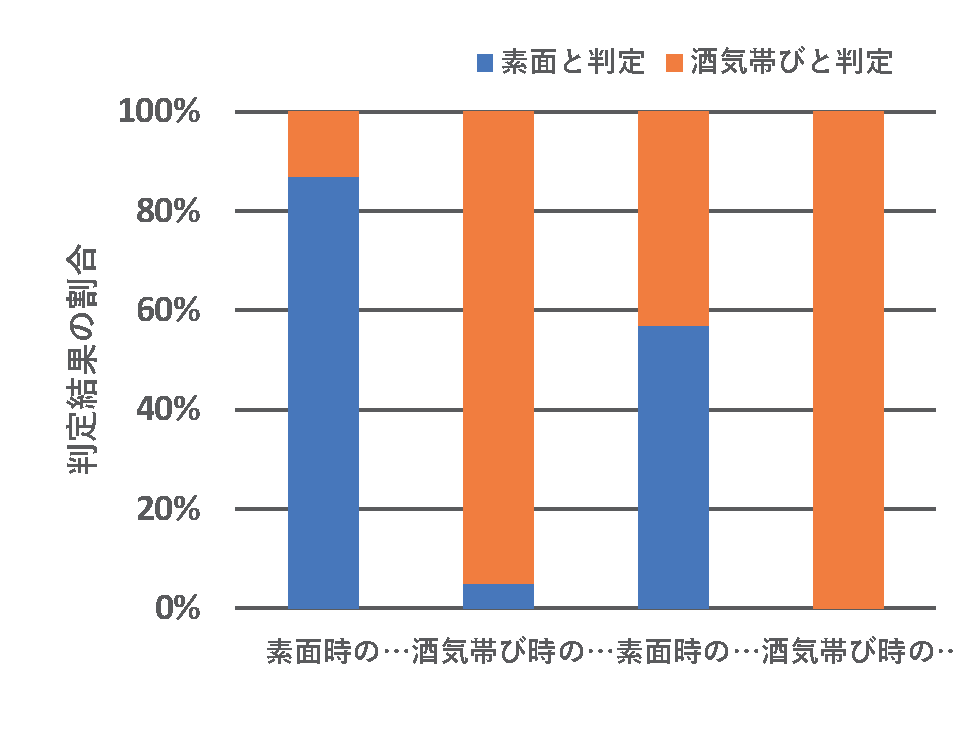
\includegraphics[width=\textwidth]{sample.eps}
    \caption{図の例．どこかにあったepsを適当に貼った}
    \label{fig:sample}
\end{figure}


\begin{table}[t]
    \caption{表の例だよ}
    \label{tab:sample2}
    \centering
    \begin{tabular}{|c||c|c|}
    \hline
     & 見出し1 & 見出し2 \\ \hline \hline
    すごい & 100 & 1000 \\ \hline
    ややすごい & 100 & 1000 \\ \hline
    とんでもない & 100 & 1000 \\ \hline
    \end{tabular}
\end{table}

\begin{figure}[t]
    \centering
    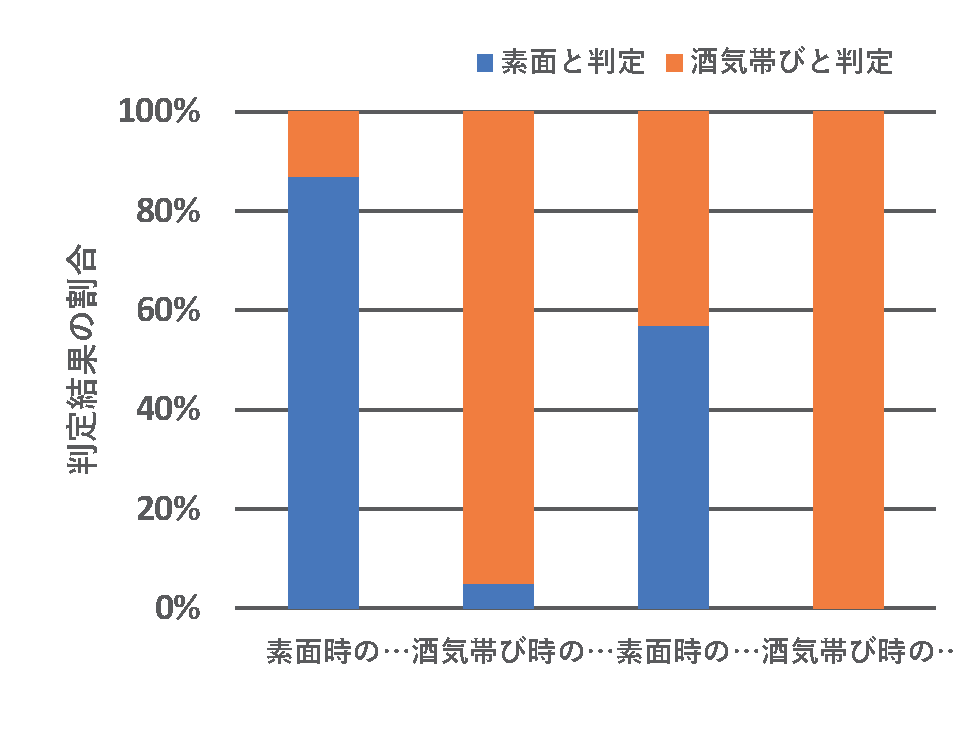
\includegraphics[width=0.7\textwidth]{sample.eps}
    \caption{図の例．どこかにあったepsを適当に貼った}
    \label{fig:sample2}
\end{figure}

\begin{table}[t]
    \caption{表の例だよ}
    \label{tab:sample3}
    \centering
    \begin{tabular}{|c||c|c|}
    \hline
     & 見出し1 & 見出し2 \\ \hline \hline
    すごい & 100 & 1000 \\ \hline
    ややすごい & 100 & 1000 \\ \hline
    とんでもない & 100 & 1000 \\ \hline
    \end{tabular}
\end{table}

\begin{figure}[t]
    \centering
    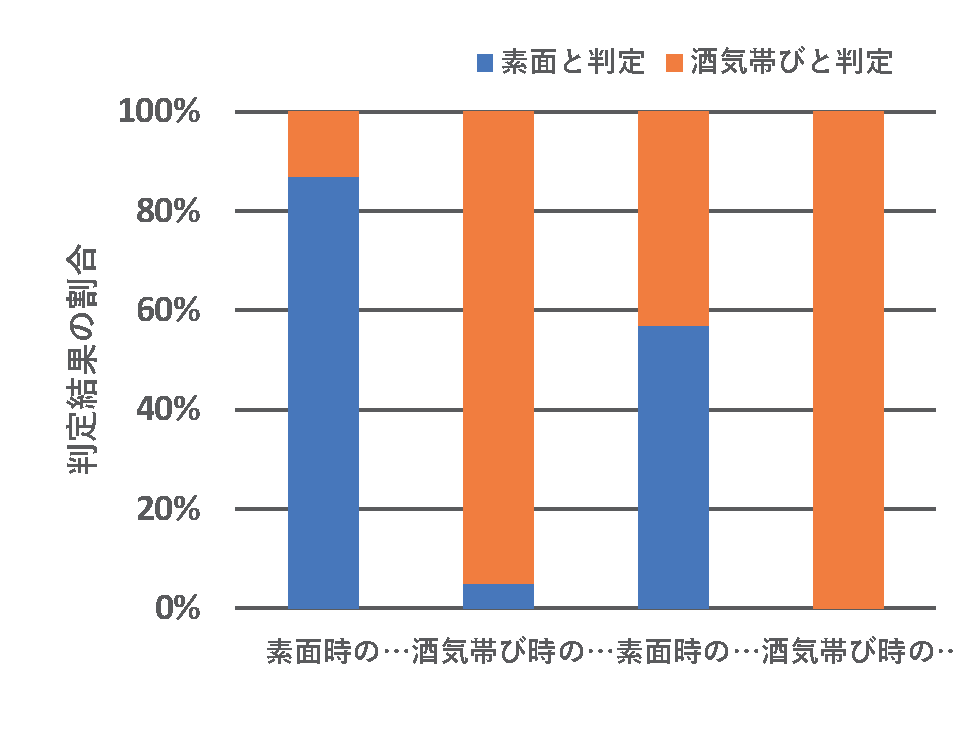
\includegraphics[width=\textwidth]{sample.eps}
    \caption{図の例．どこかにあったepsを適当に貼った}
    \label{fig:sample3}
\end{figure}

